%
%  original proposed schedule, for reference
%
\section{Management Process}
\label{sec:managementprocess}

\subsection{Project Estimates}

The MSRI award to Haystack calls for approximately one FTE of effort spread across 4 years.  In principal additional resources for testing, validation and interfacing with other resources in the EHT will be available.  (At the very least, the Calibration and Analysis working group [C\&E-WG] will be involved in specification and testing.)

\FIX[Say something to motivate these estimates?]


\subsection{Project Plan}

The notional schedule is shown in Fig.~\ref{fig:prop-quarterly}.

\begin{figure}[!h]
  \captionsetup{width=0.6\linewidth}
  \center{\fbox{%
    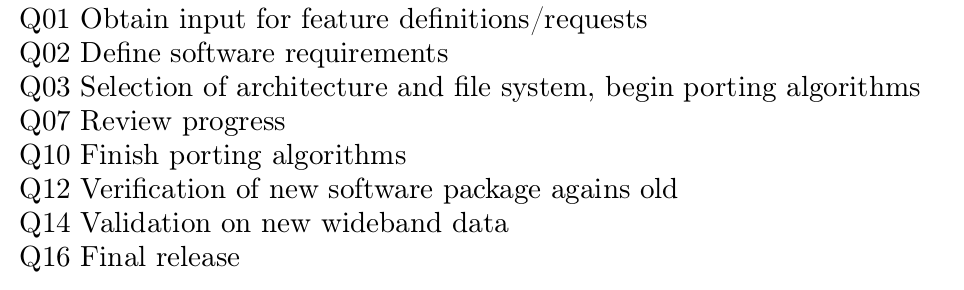
\includegraphics[width=0.70\textwidth]{nuHOPStimeline}}}
  \caption[Proposed Quarterly Plan]{This snippet from the proposal shows the original quarterly plan of develop for the ``new'' HOPS project.  Notionally the project kicked-off Oct 1, 2019, so Q1 is Oct--Jan of that year.  Notionally, then the final quarter, Q16 is July--Sep of 2023. The \ac{ngEHT} effort will need to start working on the MSRI-II proposal around Q13 (Oct-Dec 2022), so our goal for that point is to be completing whatever work is necessary to be shovel-ready for the proposal.}
\label{fig:prop-quarterly}
\end{figure}

After the proposal was accepted, the work was waterfalled into a Gantt format (see Fig.~\ref{fig:ganttcrap}) which is useful to establish that the tasks proposed are plausible for the time allowed.  The project shall be using an agile development methodology which does not lend itself to a waterfall diagram.
\begin{figure}[!h]
  \captionsetup{width=0.7\linewidth}
  \center{\fbox{%
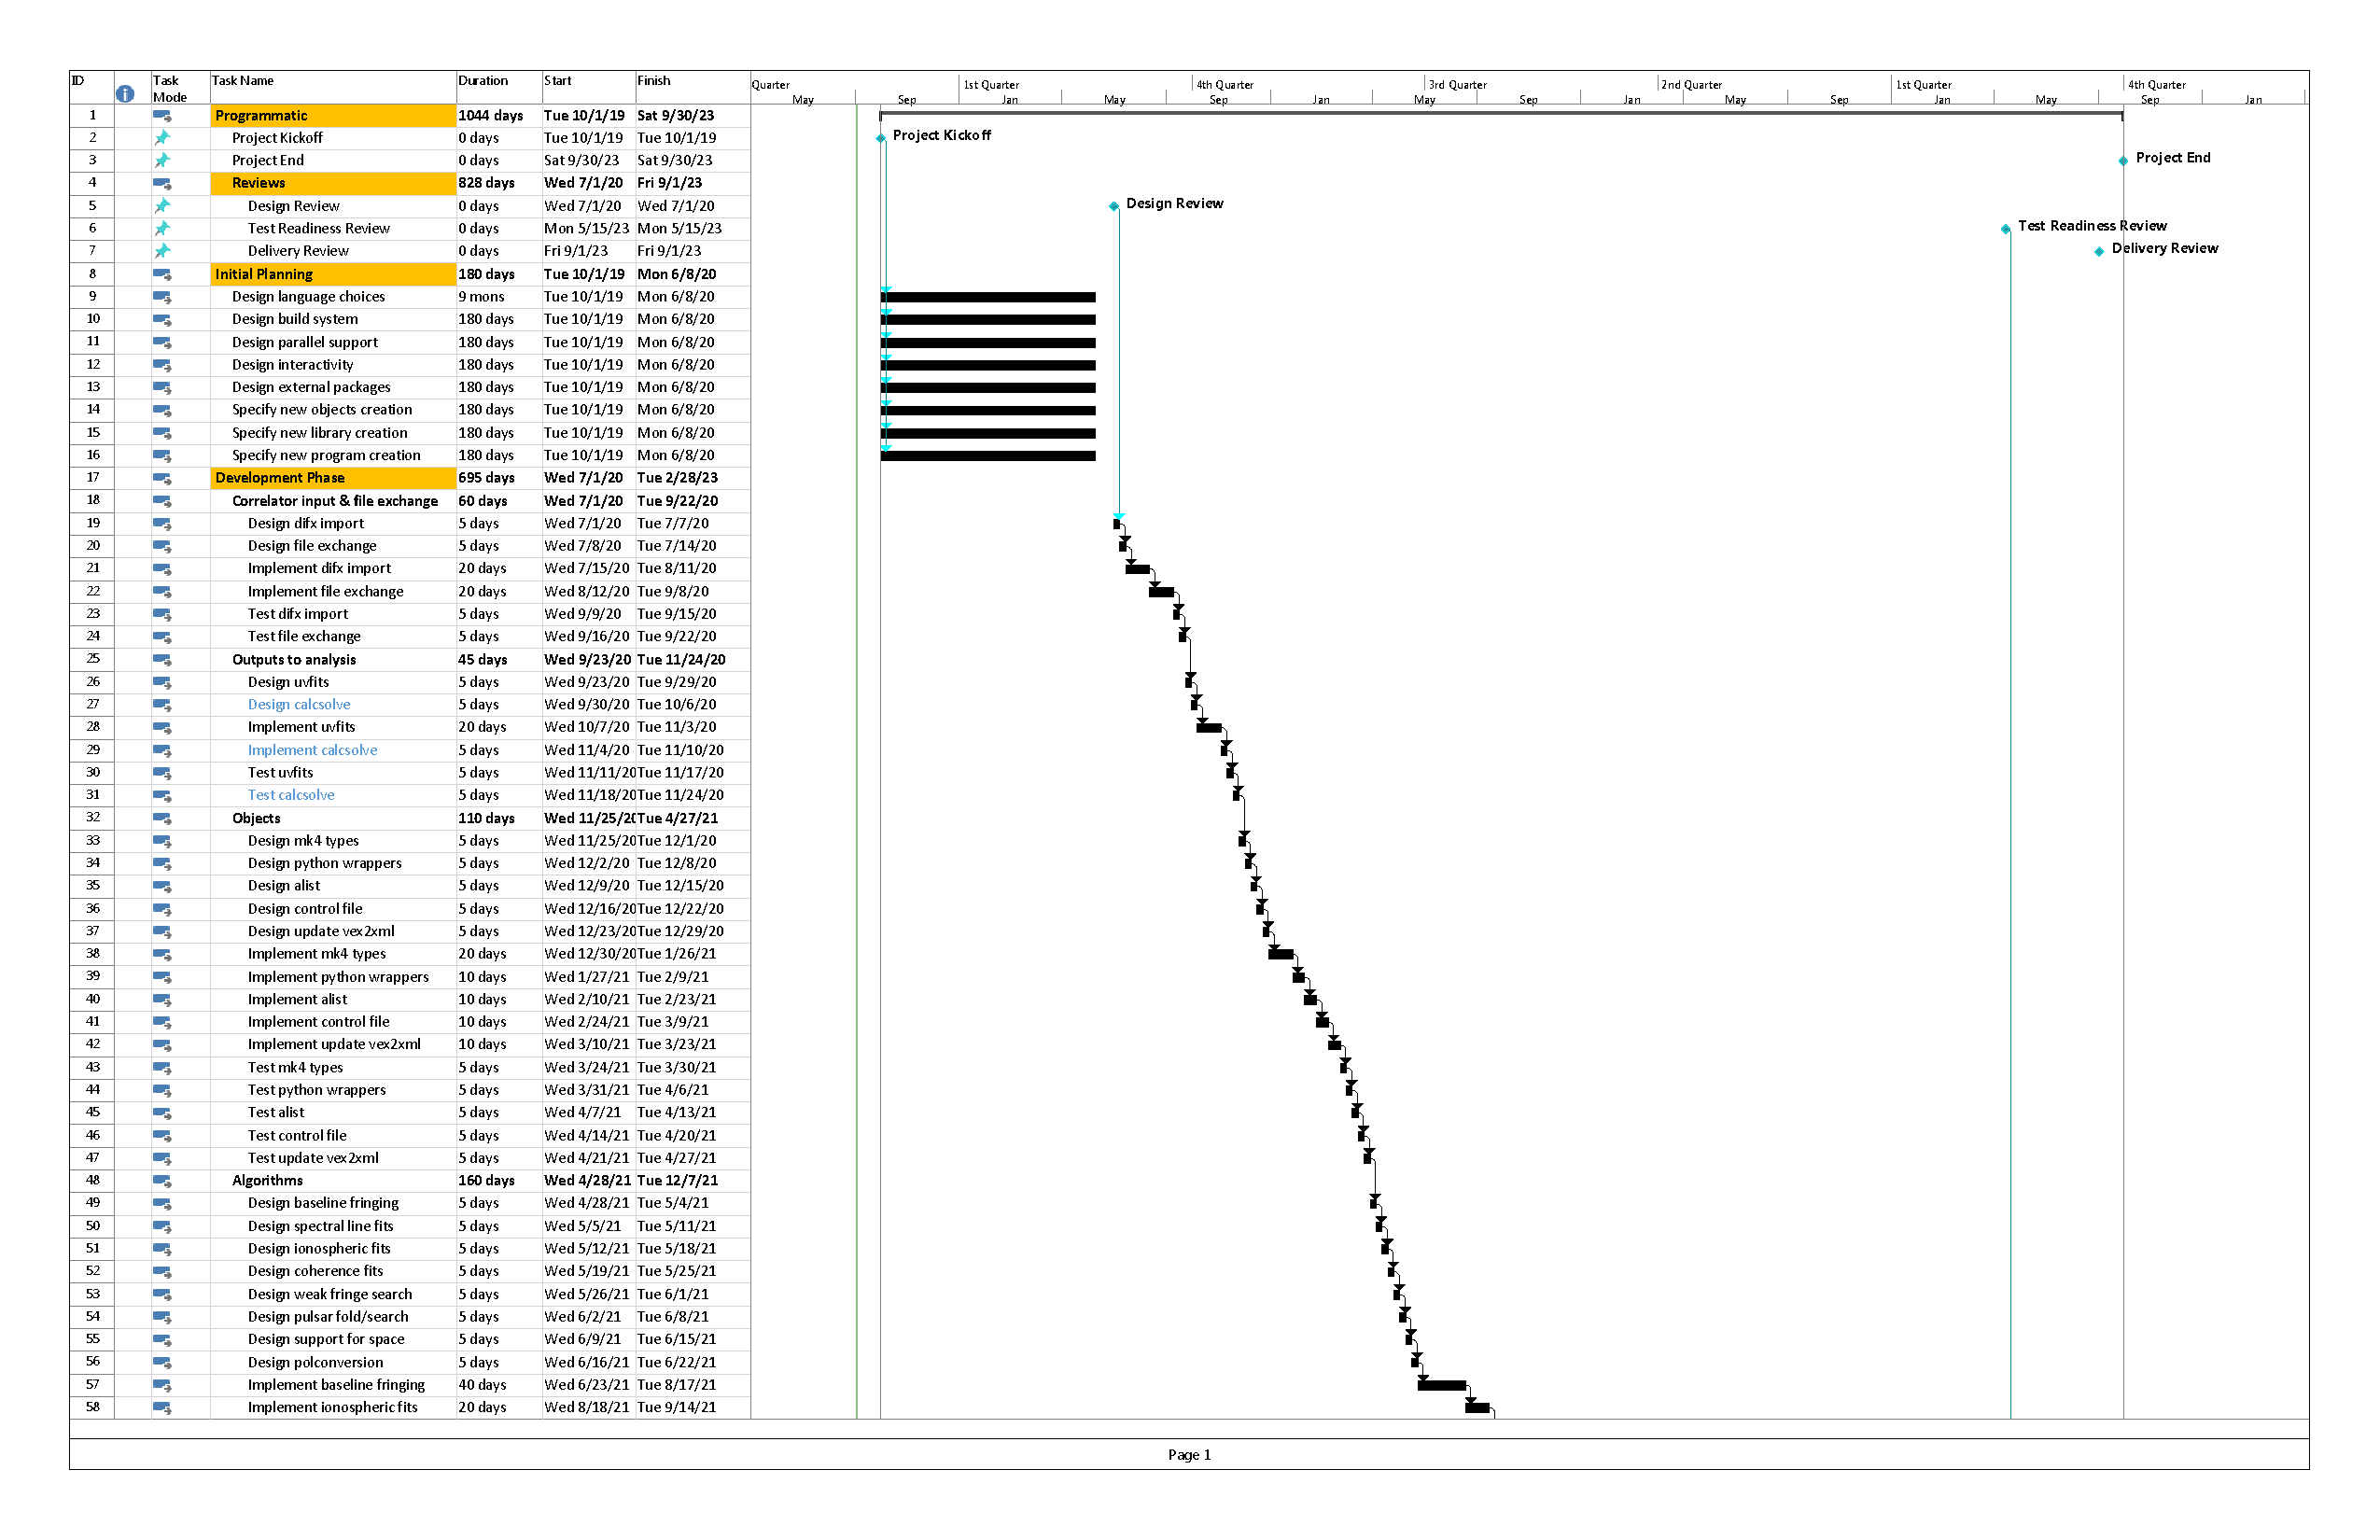
\includegraphics[width=0.40\textwidth]{MSRI-task-origv3-1}
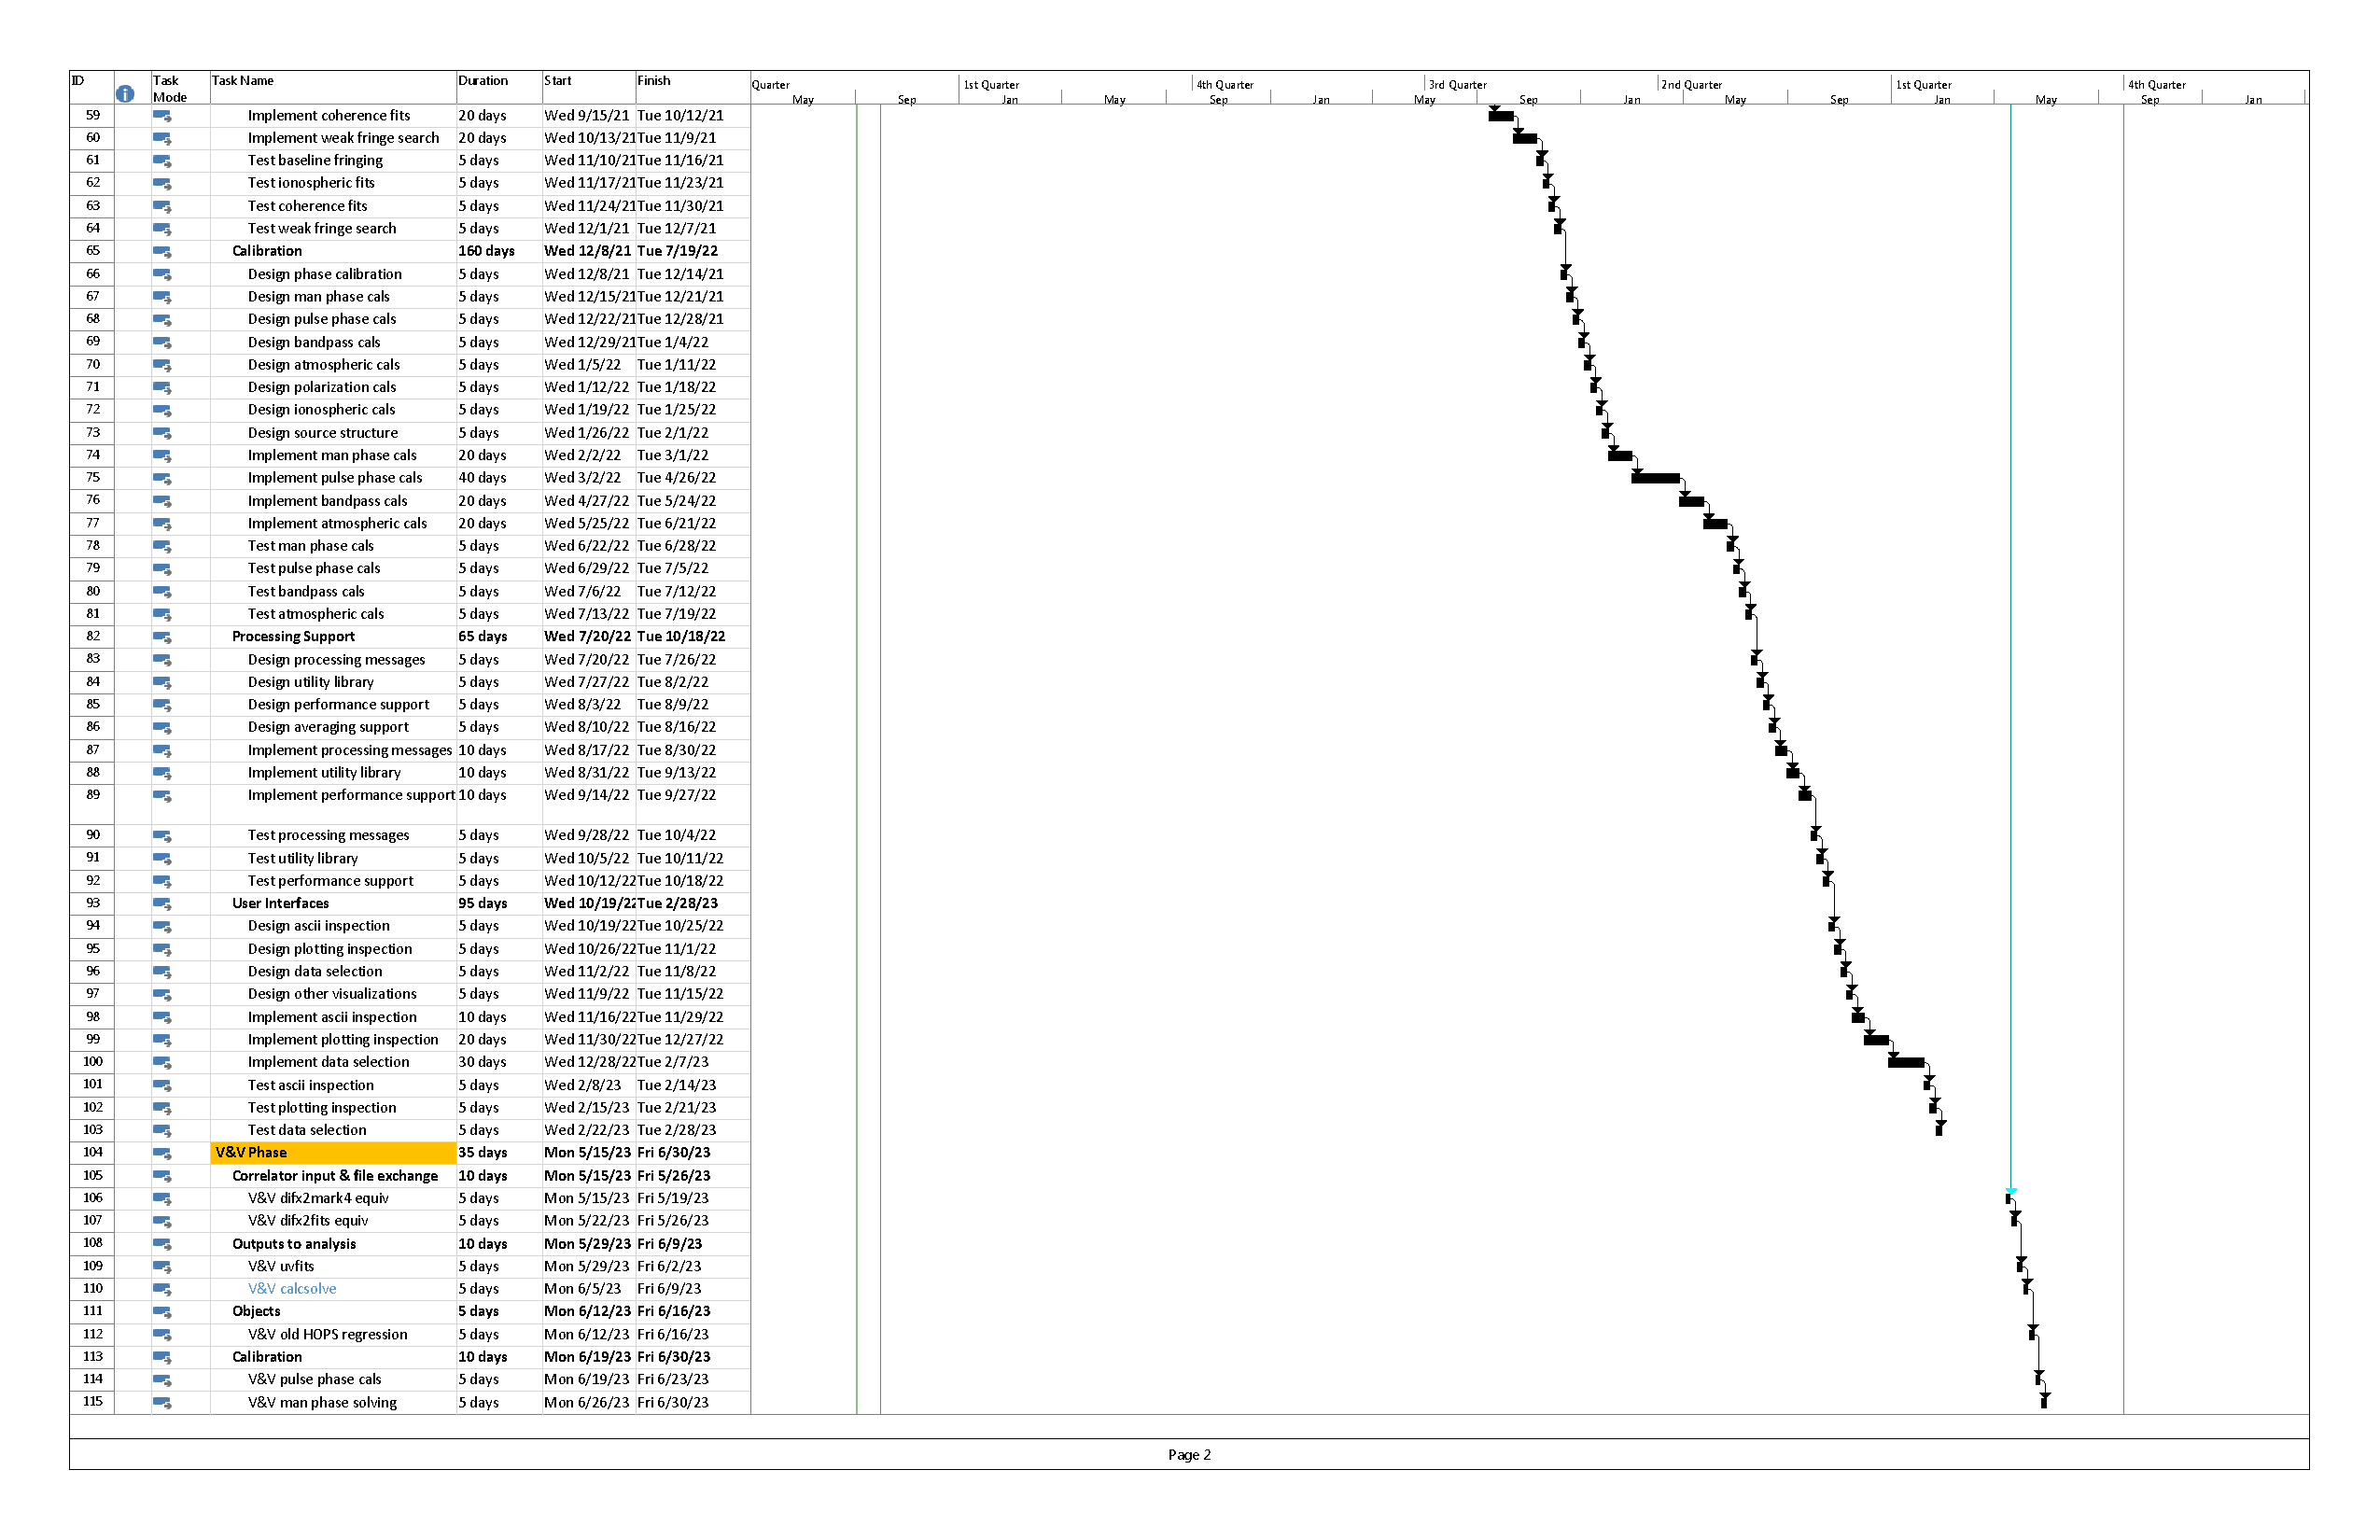
\includegraphics[width=0.40\textwidth]{MSRI-task-origv3-2} }}
\caption[Initial Gantt Timeline]{%
At the outset, a waterfalled Gantt-formulation of the work was
made to show that the 4-year timeline and estimated work effort
was consistent. The left panel corresponds to Q01--Q08, and the
right panel corresponds to Q09--Q16.}
\label{fig:ganttcrap}
\end{figure}

The COVID-19 pandemic slowed the initial stages of the project, especially the hiring of software developers (Hoak \& Pfieffer).  Nonetheless, a requirements review was held with EHT stakeholders in February 2021 (Q6 of the proposed schedule).

\subsubsection{Phase Plan}

\FIX[Define major milestones and achievement criteria; this section relies on the Detailed Timeline?]

\subsubsection{Iteration Objectives}

\FIX[Do we plan to iterate? If so:]

Iterations of the HOPS4 project will occur at points where various functionality is established. For example, the initial \texttt{fourfit} application will likely be imported from the existing HOPS3 libraries with minor reorganization; in this iteration, \texttt{fourfit} will run in HOPS4, but have the same underlying code and functionality as HOPS3. In a later release, the fourfit modules will be refactored to enable modularization of the application and extension to meet the \ac{ngEHT} requirements on stations, baselines, bands, etc.

\FIX[specify iterations? new data containers; refactoring of alist, aedit; no more PGPLOT; etc. Are iterations internal?]

\subsubsection{Releases}

\FIX[Do we plan to have releases? If so:]

HOPS4 will have a series of demo and beta releases prior to the final release, to allow stakeholders to test particular applications of the software. As a part of the agile development process, the schedule of releases is notional

\FIX[specify releases? new control file syntax, python interfaces, etc]

\subsubsection{Project Resourcing}

The current staff for the HOPS4 project (Barrett, Crew, Hoak, Pfieffer) have extensive software development experience across multiple languages (C/C++, Python, Perl, etc).  Crew and Barrett have used and maintained the exisiting HOPS package for years, and are familiar with its use-cases, functions and dependencies.

\subsection{Project Monitoring and Control}

\subsubsection{Requirements Management}

Requirements for the HOPS4 project are defined in the Requirements document. Changes to the requirements will be escalated to the project management, who will decide whether to alter the scope in order to preserve target completion dates.

\FIX[Mention requirements that may be de-scoped?]

\subsubsection{Schedule and Budget Control}

Expenses are primarily salary, which is fixed.

Schedule is monitored using the Detailed Timeline, which includes the expected duration and date for each milestone. Changes to the schedule will be escalated to the project management, who will decide whether to alter the scope in order to preserve target completion dates.

\subsubsection{Quality Control}

The HOPS4 project will have a extensive suite of tests, designed to verify the functionality of the software across the defined requirements. Existing functionality (from HOPS3) will be verified with automated check scripts using captured data.  New functions, modules and libraries will be delivered with unit tests to verify their functionality across different platforms and environments.  Furthermore, the project will use a continuous integration server to verify that the software compiles successfully after new commits, and profiling tools will be used to measure and monitor software performance (memory usage, CPU time, etc).  The details of the HOPS4 tests are described in the Coverage \& Testing document.

Defects (for example poor performance of a particular module in a particular environment) will be tracked through issues in the project git repository. 


\subsubsection{Reporting and Measurement}

The suite of HOPS4 tests shall be designed such that their output can be captured in reports. These reports will be organized to demonstrate progress towards the project requirements (\FIX[graphical trends?]). 

\subsubsection{Risk Management}

Risks are tracked by the \ac{ngEHT} management. Risks can be raised by any team member, are discussed internally at weekly meetings, and are reported and updated to \ac{ngEHT} management at monthly meetings. Risks for the HOPS4 project are primarily schedule risks, \eg that significant developer time may be needed to mitigate them.

Currently, only two risks are tracked:

\begin{itemize}

\item \textbf{Undiscovered bug in commit} A software deficiency or bug is discovered late in the project lifecycle which requires significant developer resources to correct. This may result in de-scoped requirments to remain on schedule. Continuous testing \& profiling is used to mitigate the likelihood of a serious deficiency.

\item \textbf{Incomplete ngEHT requirements} A critical use case is specified late in the project lifecycle, which requires significant developer time to extend or adapt the code. Modular code design will be used so that extensions \& restructuring are mitigated. 

\end{itemize}


\subsubsection{Configuration Management}

We use an MIT-hosted Gitlab Enterprise for tracking changes and issues.  Integration and regression tests are run on a daily or per-commit schedule.

\FIX[Do we need to mention backups?]

%
% eof
%
